\section{从一个最基本的问题出发：用散射场判断材料}
电磁逆散射要回答的是：向一个未知物体发射电磁波，在外部测量散射场，能否据此恢复物体内部的介电性质？这里未知的是材料分布，接收器直接测到的却是电场。材料和测量之间隔着一层重要的物理量——物体内部的感应电流。

可以把正向过程想成三步。入射波进入物体，材料在局部电场作用下产生感应电流；这些电流向外辐射，也会在物体内部产生新的电场；接收器记录所有这些作用叠加后的结果。材料恢复则要反过来判断：当前预测和测量之间的差异，应该通过怎样的材料变化来解释。

这也是我最初从 Gaussian/N-Port 表示出发研究这个问题的原因。其中 Gaussian basis（高斯基函数）用局部平滑函数描述材料，N-Port（有限端口表示）则把内部电流耦合组织成有限维通道关系。用有限的材料基函数和电流自由度表示三维物体，可以减少全波模型的规模。但在反演中，模型小并不是唯一要求。模型还需要准确告诉我们：材料向某个方向改动一点，测量会怎样变化。如果保留的电流可以很好地拟合当前场，却没有保留这条变化关系，材料更新仍可能受到影响。

因此，我逐渐把注意力从“如何压缩更多自由度”转向了一个更具体的问题：\textbf{一个电流模式，究竟通过什么路径影响材料更新？}这里的电流模式是一个空间分布方向，不一定是一个局部电流环，也不一定对应单一的物理谐振。

\section{已有子空间方法告诉了我们什么}
已有方法常把容易观测或对内部传播重要的电流组织成较小子空间。子空间优化方法（subspace-based optimization method，SOM）的一个基本出发点，是利用接收算子分析哪些感应电流容易被测量看到。对接收算子做奇异值分解，可以把电流方向按其辐射到接收器的能力组织起来，再结合材料与电流之间的一致性求解反演。这提供了非常清楚的物理解释：测量并不会同样敏感地看到每一种内部电流。

Twofold SOM（双重子空间优化方法，TSOM）进一步同时考虑外部观测和内部传播；FFT-TSOM（基于快速傅里叶变换的 TSOM）使用 Fourier 子空间提高构造和计算效率。子空间失真 Born 迭代方法（subspace-based distorted-Born iterative method，S-DBIM）则在更新背景场的过程中利用确定性电流信息。外部观测与内部传播的联合组织，正是这项研究的文献起点。陈教授的专著对这条方法脉络作了系统介绍。

我希望补充的角度是：\textbf{固定某一次材料状态和反演更新，指定增加一个电流方向后，材料这一步到底怎样改变？}这与寻找普遍最好的电流排序不同。它要求同时知道当前材料、当前总场、照明、接收方式和允许改变的材料方向。

这一问题也与已有的 正向/伴随降阶模型（primal/dual reduced-order model）有关。正向解描述激励怎样进入系统，伴随解描述输出怎样反向影响系统；在合适的包含条件下，两类信息可以保持输出及参数导数。这些一般思想不是新的。我的工作是把它们落实到电磁散射的电流、内部反馈和材料更新之间，寻找可以直接解释和检验的关系。

\section{反馈的直觉：接收器看到的不只是新增电流的直接辐射}
设物体中已经保留了一组电流方向，现在再加入一个方向。它可以直接向接收器辐射，也可以先在物体内部产生场，激发原来保留的电流，再由后者辐射。第二条路就是这里所说的保留空间反馈（retained feedback）。

借用反馈系统的图像，会更容易理解：新增电流把扰动送入内部回路，内部回路给出一个响应，然后接收器看到两条路的叠加。这里讨论的是频域多重散射方程，并没有另行设计一个时域控制器；反馈也不意味着响应总被放大。电磁场有相位，直接响应与反馈响应可以增强，也可以抵消。

\begin{figure}[htbp]\centering
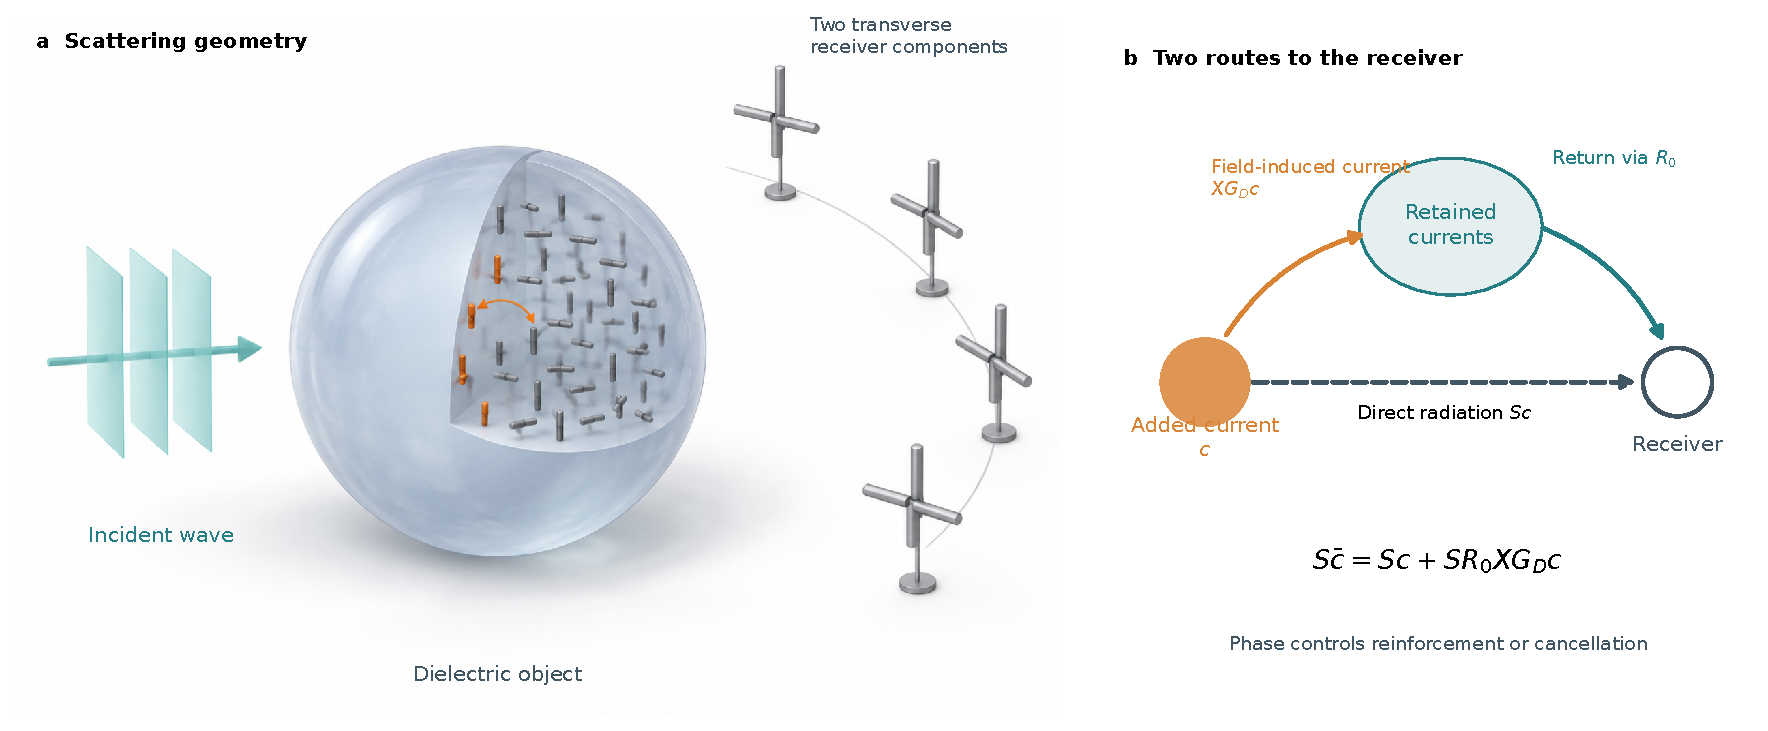
\includegraphics[width=\linewidth]{figures/physical_feedback.pdf}
\caption{新增电流存在两条到达接收器的路径：直接辐射，以及经过保留电流的内部反馈。物体和天线为概念示意，不代表某次计算的场分布。}
\end{figure}

这一点对弱辐射电流尤其重要。即使一个方向的直接接收输出很小，若允许的材料变化能激发它，并且它能经内部耦合返回接收通道，材料导数仍可能受到明显影响。因此，“直接看不见”与“对材料更新无影响”并不是同一件事。

